\documentclass[11pt,a4paper]{article}
\usepackage[T1]{fontenc}
\usepackage[margin=2.3cm]{geometry}
\usepackage{amsmath,amssymb}
\usepackage{graphicx}
\usepackage[dvipsnames]{xcolor}
\usepackage{enumitem}
\usepackage[colorlinks=true,linkcolor=blue,urlcolor=blue]{hyperref}
\setlength{\parskip}{0.6em}
\setlength{\parindent}{0pt}
\begin{document}

\begin{center}{\LARGE\bfseries opencncpath}\\[0.4em]{\large Turn a drawing into a CNC toolpath, in three sessions.}\\[0.2em]\small PAN IIT OSS explainer \textbullet{} diploma / undergraduate to advanced undergraduate (levels 5-6)\end{center}

\section*{Why this exists}
Every machined part starts as a drawing and ends as a list of coordinates that a cutter follows. This explainer shows the geometry in between, offsets, arcs, stepovers and a height-map check, using only simple formulas, so you can build it yourself.

\section*{The end goal}
Turn a drawing into a CNC toolpath. The end goal is to turn a drawing into a CNC toolpath: the planning step that CAM software does for machining. This repo teaches the geometry only; real machining needs trained operators, machine-specific post-processing and safety checks.

\section*{How the three sessions build up}
\begin{enumerate}[nosep]
\item \textbf{Session 1: A cutter follows a path} (Level 1, conceptual interactive model, 60 min).
\item \textbf{Session 2: G-code, offsets and arcs} (Level 2, mathematical engineering model, 75 min).
\item \textbf{Session 3: Pocketing strategies and a simulation that checks them} (Level 3, simulation and validation, 90 min).
\end{enumerate}

\section{Session 1: A cutter follows a path}

\subsection*{A. Real-world problem}
A plotter draws by moving a pen to coordinates. A CNC (computer numerical control) milling machine does the same with a spinning cutter that carves material instead of ink. To carve a square pocket, the machine needs a list of points for the cutter centre, not for the wall. Where must the centre go so that the cutter edge just touches the wall, and how long does one lap take? Educational geometry only: real machining needs trained operators, machine-specific post-processing and safety checks.

\subsection*{B. Concept and theory}
The cutter is a disc of diameter d, radius r = d/2, seen from above. If its edge must touch the wall, its centre must stay r away from the wall: the centre path is the wall moved inwards by r, a smaller square of side (side - 2r) = (side - d). The disc removes everything within r of its centre, so one lap clears a strip of width 2r = d along each wall (the four inside corners stay slightly rounded). What is left in the middle is an island, a square of side (side - 4r) = (side - 2d) if that is positive. The feed F is the speed along the path in mm per minute, so a path of length L takes L / F minutes.

\begin{itemize}[nosep]
\item side: side of the square pocket (mm)
\item d: cutter diameter (mm)
\item r: cutter radius, d/2 (mm)
\item F: feed rate (speed along the path) (mm/min)
\item L: length of the cutter-centre path (mm)
\item t: time for the path (s)
\end{itemize}

\begin{equation*}
r=\frac d2,\qquad L=4\,(\text{side}-d)
\end{equation*}

\begin{equation*}
t=\frac{L}{F}\cdot 60\ \text{s}\quad(F\ \text{in mm/min})
\end{equation*}

\begin{equation*}
\text{island side}=\max(0,\ \text{side}-4r)=\max(0,\ \text{side}-2d)
\end{equation*}

\begin{center}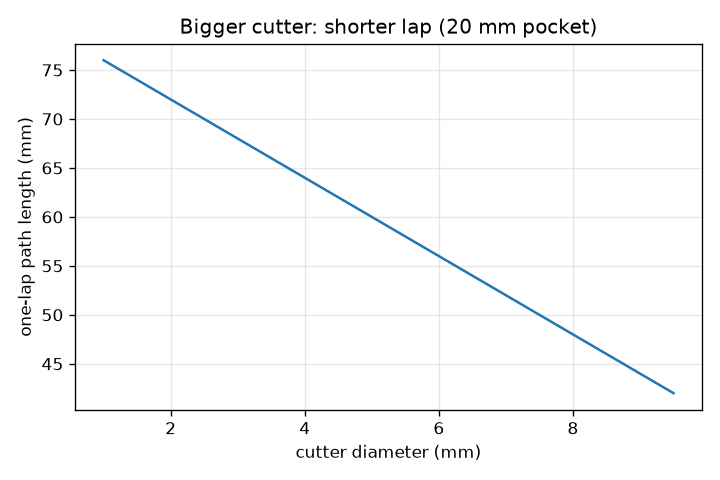
\includegraphics[width=0.85\linewidth]{figures/s01_lap_length_vs_diameter.png}\\\small One-lap path length against cutter diameter for a 20 mm pocket.\end{center}

\subsection*{E. Worked example}
A 20 mm square pocket is cut with a 4 mm cutter at 120 mm/min. Find the centre path, its length, the time for one lap and the island that is left.
\begin{enumerate}[nosep]
\item Radius r = 4 / 2 = 2 mm. The centre path is the square from 2 mm to 18 mm in x and y, with side 16 mm.
\item Length L = 4 * 16 = 64 mm.
\item Time = 64 / 120 min = 0.533 min = 32.0 s.
\item Island side = 20 - 4 * 2 = 12 mm: a 12 mm square in the middle is not touched.
\end{enumerate}
\textbf{Answer.} The cutter centre follows a 16 mm square (64 mm long); one lap takes 32.0 s and leaves a 12 mm square island.

\subsection*{F. Questions}
\begin{enumerate}[nosep]
\item \textbf{Conceptual.} Why does the cutter centre have to follow a path one radius inside the wall, and why does one lap of a big pocket leave an island?
\item \textbf{Numerical.} A 30 mm square pocket is cut with a 6 mm cutter at 150 mm/min. Find the path length, the time for one lap and the island side.
\item \textbf{Graph and simulation interpretation.} In the time graph the curve falls as the feed rises. If the feed is halved from 120 to 60 mm/min for the 64 mm path, what happens to the time? What does the curve shape say?
\item \textbf{Design and optimisation challenge.} Design: choose a cutter diameter and a feed to clear a 20 mm pocket in one lap, with no island, in under 20 s. Is there a limit on the feed?
\end{enumerate}

\section{Session 2: G-code, offsets and arcs}

\subsection*{A. Real-world problem}
A CNC controller reads text such as \texttt{G1 X10 Y5 F300}. You will write that text with a tiny Python generator, read it back to check the geometry, and use it to plan a pocket: a 40 x 30 mm pocket, 5 mm deep, with a 6 mm cutter taking at most 2 mm depth per pass. How many passes and lines are needed, and how long will it take? Educational toolpath geometry only: real machining needs trained operators, machine-specific post-processing and safety checks.

\subsection*{B. Concept and theory}
A G-code line is a list of words, each a letter and a number. G0 is a rapid move (not cutting) and G1 a straight cutting move; X, Y, Z are target coordinates in mm (G21 mm, G90 absolute); F is the feed in mm/min. G2 is a clockwise and G3 a counter-clockwise circular arc to (X, Y); I and J are the offsets from the START point to the arc centre, so the centre is (x0 + I, y0 + J). A valid arc has the same radius sqrt(I\textasciicircum{}2 + J\textasciicircum{}2) at the start and at the end, and its length is the radius times the swept angle in radians. Words are modal: a missing coordinate, the G word and F keep their last values. The toolpath is an offset curve of the part outline: for a pocket the cutter centre follows the outline moved inwards by r (a w x h rectangle becomes (w - 2r) x (h - 2r)); for a profile around a part it follows the outline moved outwards by r, and the rectangle's corners become arcs of radius r. A pocket is cleared with zigzag lines along x spaced by at most the stepover s, in layers of at most the depth of cut. The time is the cutting length divided by the feed, plus the plunge.

\begin{itemize}[nosep]
\item X, Y, Z: target coordinates (absolute) (mm)
\item F: feed rate (mm/min)
\item I, J: arc centre minus arc start (mm)
\item r: cutter radius (D/2) (mm)
\item D: cutter diameter (mm)
\item s: stepover between lines (mm)
\item n: number of zigzag lines (no unit)
\item N: number of depth layers (no unit)
\item doc: depth of cut per layer (mm)
\item T: machining time (s)
\end{itemize}

\begin{equation*}
T=\frac{L}{F}\cdot 60\ \text{s}\quad(L\ \text{in mm},\ F\ \text{in mm/min})
\end{equation*}

\begin{equation*}
\text{centre}=(x_0+I,\ y_0+J),\qquad R=\sqrt{I^2+J^2},\qquad L_{\text{arc}}=R\,\theta
\end{equation*}

\begin{equation*}
\text{pocket path: }(w-D)\times(h-D),\qquad \text{profile path: }(w+D)\times(h+D)\ \text{with corner arcs of radius }r
\end{equation*}

\begin{equation*}
n=\left\lceil\frac{h-D}{s}\right\rceil+1,\qquad N=\left\lceil\frac{\text{depth}}{doc}\right\rceil,\qquad L_{\text{layer}}=n\,(w-D)+(h-D)
\end{equation*}

\begin{equation*}
T=\frac{N\,L_{\text{layer}}}{F}\cdot 60+\frac{\text{depth}+0.5}{F_{\text{plunge}}}\cdot 60
\end{equation*}

\begin{center}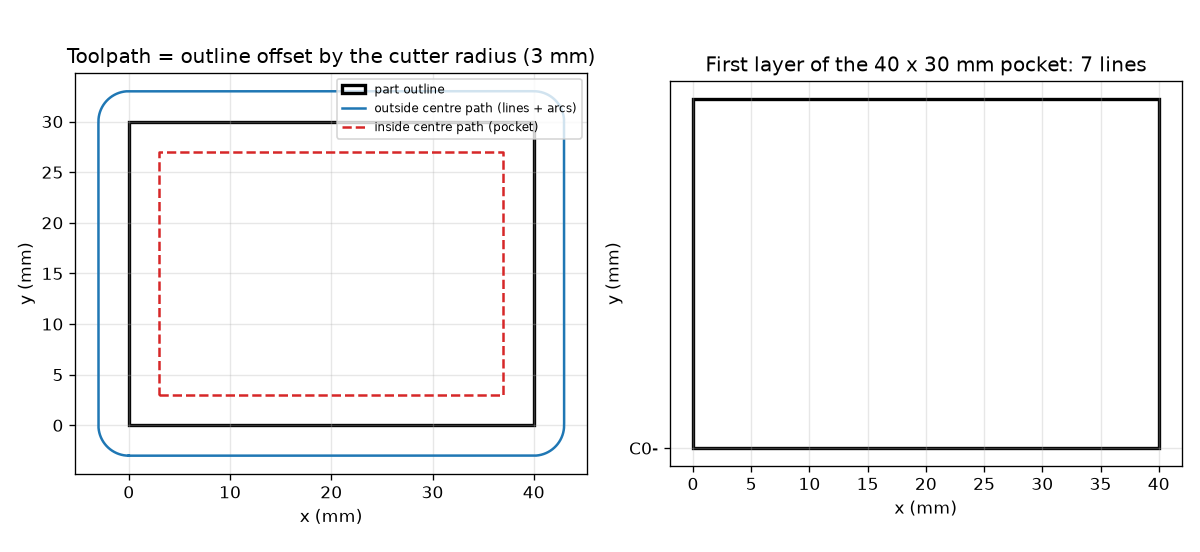
\includegraphics[width=0.85\linewidth]{figures/s02_offsets_and_pocket.png}\\\small Offsets of a 40 x 30 mm outline by 3 mm (pocket inside, profile outside with corner arcs) and the first layer of the pocket.\end{center}

\subsection*{E. Worked example}
Design: clear a 40 x 30 mm pocket, 5 mm deep, with a 6 mm cutter and a 2 mm depth of cut per pass at 300 mm/min. Choose the stepover and the number of passes and estimate the time.
\begin{enumerate}[nosep]
\item The centre must cover (40 - 6) x (30 - 6) = 34 x 24 mm, so lines run 34 mm long and cover a 24 mm span.
\item Choose the stepover at most 75 percent of the diameter: 4.5 mm. Lines n = ceil(24 / 4.5) + 1 = 7, spaced evenly at 24 / 6 = 4.0 mm.
\item Layers N = ceil(5 / 2) = 3, each 5 / 3 = 1.667 mm deep.
\item One layer: 7 * 34 + 24 = 262 mm; three layers: 786 mm.
\item Cutting time = 786 / 300 min = 2.62 min = 157.2 s. Plunge: 5.5 mm / 100 mm/min = 3.3 s. Total 160.5 s.
\item Parsing our own G-code gives the same 160.5 s for cutting and plunging; adding rapids at 3000 mm/min gives 162.6 s.
\end{enumerate}
\textbf{Answer.} Stepover 4.5 mm (7 lines, 4 mm apart), 3 layers, 786 mm of cutting: about 160.5 s, or 162.6 s with rapids.

\subsection*{F. Questions}
\begin{enumerate}[nosep]
\item \textbf{Conceptual.} The same start (10, 0) and end (0, 10) with I-10 J0 are used for G3 and for G2. Do they give the same arc? Why does the centre not change?
\item \textbf{Numerical.} An arc starts at (20, 0), ends at (0, 20) and is written G3 X0 Y20 I-20 J0. Find the centre, check the end radius and find the arc length.
\item \textbf{Graph and simulation interpretation.} On the time-against-stepover graph, the time is 282.9 s at a stepover of 2 mm and 119.7 s at 6 mm. Why does the curve fall quickly at first and then flatten? Why can the stepover not exceed 6 mm?
\item \textbf{Design and optimisation challenge.} Design: repeat the plan with an 8 mm cutter (stepover at most 75 percent of D, depth of cut 2 mm, 300 mm/min, plunge 100 mm/min). How many lines, how much cutting length and what time? Is it faster than the 6 mm cutter, and what is the catch?
\end{enumerate}

\section{Session 3: Pocketing strategies and a simulation that checks them}

\subsection*{A. Real-world problem}
A toolpath that looks right can still leave material behind, cut too much, or take twice as long as it should. We cut a simulated block on a grid of heights (a height-map), subtract the cutter footprint along the path, and compare the removed volume and the leftover ridges with formulas. At the end we generate G-code for a pocket with a round boss and check its removed volume. Educational toolpath geometry only: real machining needs trained operators, machine-specific post-processing and safety checks; the feeds and speeds here are teaching numbers.

\subsection*{B. Concept and theory}
The height-map stores the height of the material top in each grid cell (0 = original top). A flat-end cutter at (x, y) with tip height z sets every cell within its radius to at most z; a ball-end cutter of radius r leaves height z + r - sqrt(r\textasciicircum{}2 - rho\textasciicircum{}2) at distance rho from its axis. Raster pocketing uses parallel lines; contour-parallel pocketing offsets the outline inwards by r, r + s, r + 2s, and so on. Neighbouring ball-end passes s apart leave a ridge midway of height h = r - sqrt(r\textasciicircum{}2 - (s/2)\textasciicircum{}2); inversely s = 2 sqrt(2 r h - h\textasciicircum{}2). The material removal rate is MRR = a\_e a\_p F (radial width, axial depth, feed) and the chip load is f\_z = F / (N z) for N rev/min and z teeth. A round flat cutter cannot reach into a sharp inside corner: each of the four corners keeps r\textasciicircum{}2 (1 - pi/4) of area, so the pocket keeps 4 r\textasciicircum{}2 (1 - pi/4). A stepover larger than the cutter diameter D leaves strips of width s - D. An offset in the wrong direction makes the cutter cut outside the pocket. A slot narrower than the cutter cannot be cut, and the planner must report that.

\begin{itemize}[nosep]
\item r: cutter radius (mm)
\item s: stepover between passes (mm)
\item h: ridge (scallop) height (mm)
\item a\_e: radial width of cut (mm)
\item a\_p: axial depth of cut (mm)
\item F: feed rate (mm/min)
\item N: spindle speed (rev/min)
\item z: number of cutting teeth (no unit)
\item f\_z: chip load, feed per tooth (mm)
\item MRR: material removal rate (mm\textasciicircum{}3/min)
\end{itemize}

\begin{equation*}
h=r-\sqrt{r^{2}-\left(\frac s2\right)^{2}},\qquad s=2\sqrt{2rh-h^{2}}
\end{equation*}

\begin{equation*}
\mathrm{MRR}=a_e\,a_p\,F,\qquad f_z=\frac{F}{N\,z}
\end{equation*}

\begin{equation*}
A_{\text{corners}}=4\,r^{2}\left(1-\frac{\pi}{4}\right)
\end{equation*}

\begin{equation*}
A_{\text{gouge}}=(w+4r)(h+4r)-(4-\pi)r^{2}-wh\quad(\text{centre path offset outwards by } r)
\end{equation*}

\begin{equation*}
V=\left(wh-\pi R_b^{2}-4r^{2}\left(1-\tfrac{\pi}{4}\right)\right)\,\text{depth}\quad(\text{pocket with a boss of radius } R_b)
\end{equation*}

\begin{center}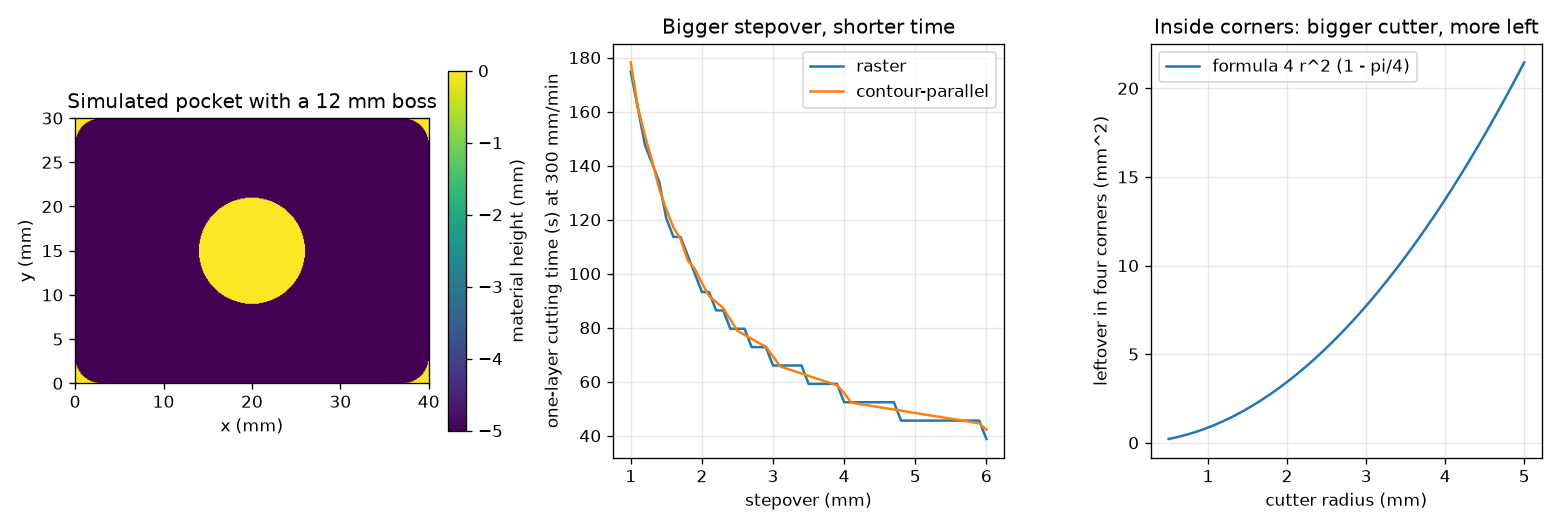
\includegraphics[width=0.85\linewidth]{figures/s03_boss_and_tradeoffs.png}\\\small Simulated boss pocket, one-layer time against stepover for two strategies, and the corner leftover against the cutter radius.\end{center}

\subsection*{E. Worked example}
A ball-end cutter of radius 3 mm makes parallel passes 2 mm apart. Find the ridge height, then the largest stepover that keeps the ridge at 0.05 mm or less, and check by simulation.
\begin{enumerate}[nosep]
\item h = 3 - sqrt(3\textasciicircum{}2 - 1\textasciicircum{}2) = 3 - sqrt(8) = 3 - 2.828 = 0.1716 mm.
\item For h = 0.05 mm: s = 2 sqrt(2 * 3 * 0.05 - 0.05\textasciicircum{}2) = 2 sqrt(0.2975) = 2 * 0.5454 = 1.0909 mm.
\item Use s = 1.0 mm (a convenient value below the limit): h = 3 - sqrt(9 - 0.25) = 0.0420 mm. With 1.1 mm the ridge is 0.0508 mm, just too high.
\item The height-map simulation of 5 passes at 2 mm gives 0.1716 mm (and 0.0420 mm at 1 mm), equal to the formula to better than 0.002 mm.
\end{enumerate}
\textbf{Answer.} Ridge 0.1716 mm at 2 mm stepover; to stay at 0.05 mm or less use at most 1.0909 mm, for example 1.0 mm (ridge 0.0420 mm). The simulation agrees.

\subsection*{F. Questions}
\begin{enumerate}[nosep]
\item \textbf{Conceptual.} Why does a bigger stepover finish a job faster but leave more material behind? Why does the contour-parallel path with stepover equal to the diameter still leave cusps in the corners?
\item \textbf{Numerical.} A cutter has 2 teeth, runs at 8000 rev/min and feeds at 480 mm/min. Find the chip load. Then find the MRR for a\_e = 3 mm, a\_p = 1.5 mm and F = 400 mm/min.
\item \textbf{Graph and simulation interpretation.} In the corner-leftover graph, read the leftover area for a cutter radius of 3 mm and of 5 mm. What happens when the radius doubles, and what does that say about choosing a cutter?
\item \textbf{Design and optimisation challenge.} Design: a ball-end cutter of radius 4 mm must finish a 40 x 30 mm face with a ridge of at most 0.02 mm at 600 mm/min. Choose a stepover (rounded down to 0.01 mm), count the lines and estimate the time. Lines run along the 40 mm side, plus 30 mm of side-steps in total.
\end{enumerate}

\section{Real-world mini-project}
\textbf{Generate G-code for a pocket with a boss and check it.} A 40 x 30 mm pocket, 5 mm deep, has a round boss of diameter 12 mm in the middle at (20, 15) that must stay. Use a 6 mm flat cutter, 2 mm depth of cut per layer, stepover 4 mm, feed 300 mm/min, plunge 100 mm/min and rapids at 3000 mm/min. Use \texttt{boss\_pocket\_gcode} from Session 3, parse the text back with \texttt{read\_moves}, simulate it on a height-map with \texttt{simulate\_moves}, and compare the removed volume with the analytic volume.

\section{The path ahead}
\begin{enumerate}[nosep]
\item \textbf{Session 4: Offset any convex polygon.} A function that returns the inward offset of a convex polygon and a pocket path for a hexagon.
\item \textbf{Session 5: Contour-parallel pocket with a boss.} A planner that clears the boss pocket with continuous rings and one plunge per layer.
\item \textbf{Session 6: Rest machining of the corners.} A second pass with a 2 mm cutter that follows the corner leftover left by the 6 mm cutter.
\item \textbf{Session 7: 3D ball-end finishing.} Parallel finishing passes over a hemisphere of radius 15 mm with a ball cutter of radius 3 mm, simulated on a 3D height-map.
\item \textbf{Session 8: Post-processor dialects.} A writer that outputs arcs with I, J and with the R word, and a parser that reads both.
\end{enumerate}

\section{Answers and hints}

\subsection*{Session 1}
\begin{enumerate}[nosep]
\item \textbf{Conceptual.} Hint: Where is the cutter edge relative to its centre? How far from the path does the cutter reach? Solution: The cutter edge is one radius from its centre, so for the edge to touch the wall the centre must be one radius from the wall. The cutter only removes material within one radius of its centre, so a single lap clears a strip of width 2r = d along the wall; if the pocket is wider than 4r, the middle is out of reach and remains as an island.
\item \textbf{Numerical.} Hint: L = 4 (side - d); t = L / F * 60; island = side - 2d. Solution: L = 4 * (30 - 6) = 96 mm. Time = 96 / 150 * 60 = 38.4 s. Island side = 30 - 12 = 18 mm. Sanity check: a bit more than 3 times the pocket side for the path, and a slow feed (150 mm/min is 2.5 mm per second) gives tens of seconds.
\item \textbf{Graph and simulation interpretation.} Hint: t = L / F * 60. Solution: The time doubles from 32 s to 64 s. The curve is a hyperbola (time inversely proportional to feed): steep at low feeds, flat at high feeds, so the first increases in feed save the most time.
\item \textbf{Design and optimisation challenge.} Hint: No island needs side \textless{}= 2d. Then t = 4 (side - d) / F * 60 \textless{} 20. Solution: Side \textless{}= 2d needs d \textgreater{}= 10 mm; take d = 10 mm. The path is 4 * (20 - 10) = 40 mm. Time under 20 s needs F above 40 / 20 * 60 = 120 mm/min (exactly 20.0 s at 120); choose 200 mm/min for 12.0 s. Trade-off: the biggest cutter and a faster feed save time, but real cutters have a maximum feed set by the machine, the material and the cutter, and a 10 mm cutter cannot cut an inside corner sharper than 5 mm radius.
\end{enumerate}

\subsection*{Session 2}
\begin{enumerate}[nosep]
\item \textbf{Conceptual.} Hint: I and J are measured from the start point. Which way round does each word go? Solution: The centre is (10 - 10, 0 + 0) = (0, 0) for both, because it depends only on the start and on I, J. G3 goes counter-clockwise and sweeps 90 degrees (length 15.708 mm); G2 goes clockwise the long way round and sweeps 270 degrees (length 47.124 mm). The endpoints are the same but the arcs are not.
\item \textbf{Numerical.} Hint: centre = start + (I, J); length = R * angle. Solution: Centre = (20 - 20, 0 + 0) = (0, 0). Start radius = 20 mm; end radius = sqrt(0 + 400) = 20 mm, so the arc is valid. Counter-clockwise from 0 to 90 degrees is pi/2 radians, so the length is 20 * pi/2 = 31.416 mm. Units: mm.
\item \textbf{Graph and simulation interpretation.} Hint: Count lines: n = ceil(24 / s) + 1. What does the cutter diameter limit? Solution: Time is mostly the number of lines times the line length, and n falls like 1 / s: halving the stepover roughly doubles the lines, but at large s the lines cannot drop below a few (5 lines at 6 mm). Because n is a whole number the curve also has small steps. The stepover cannot exceed the cutter diameter (6 mm) because then the strip between two lines is wider than the cutter and stays uncut.
\item \textbf{Design and optimisation challenge.} Hint: Span = 30 - 8 = 22 mm; line length = 40 - 8 = 32 mm; stepover at most 6 mm. Solution: n = ceil(22 / 6) + 1 = 5 lines, spaced 5.5 mm. One layer: 5 * 32 + 22 = 182 mm; three layers 546 mm. Time = 546 / 300 * 60 + 3.3 = 109.2 + 3.3 = 112.5 s, faster than 160.5 s. Catch: a bigger cutter rounds the inside corners with a larger radius (4 mm instead of 3 mm), needs more force and may exceed what the machine can hold; Session 3 measures the corner leftover.
\end{enumerate}

\subsection*{Session 3}
\begin{enumerate}[nosep]
\item \textbf{Conceptual.} Hint: Count lines. Then think about where two offset rings meet at a rectangle corner. Solution: A bigger stepover needs fewer lines, so the path is shorter and the time smaller, but the ridge between lines grows (for a ball end) and above the diameter whole strips are left. In contour-parallel paths the rings at a rectangle corner meet at 90 degrees; the round cutter covers a rounded patch, and with spacing equal to the diameter (6 mm for a 3 mm radius) the corner of the next ring is out of reach in the diagonal direction: the simulation clears only 1180.9 mm\textasciicircum{}2 instead of 1192.3 mm\textasciicircum{}2.
\item \textbf{Numerical.} Hint: f\_z = F / (N z); MRR = a\_e a\_p F. Solution: f\_z = 480 / (8000 * 2) = 0.03 mm per tooth. MRR = 3 * 1.5 * 400 = 1800 mm\textasciicircum{}3/min. Units: mm/min divided by rev/min times teeth gives mm per tooth; mm * mm * mm/min gives mm\textasciicircum{}3/min. These are teaching numbers, not recommended cutting conditions.
\item \textbf{Graph and simulation interpretation.} Hint: The curve is 4 r\textasciicircum{}2 (1 - pi/4). Solution: About 7.73 mm\textasciicircum{}2 at 3 mm and 21.46 mm\textasciicircum{}2 at 5 mm. The curve rises with the square of r: doubling the radius quadruples the leftover (3.43 mm\textasciicircum{}2 at r = 2 and 13.73 mm\textasciicircum{}2 at r = 4 also follow the formula). A bigger cutter clears faster but leaves bigger corner fillets, so a smaller cutter is needed to finish the corners (rest machining).
\item \textbf{Design and optimisation challenge.} Hint: Use s = 2 sqrt(2 r h - h\textasciicircum{}2), then n = ceil(30 / s) + 1 and length = 40 n + 30. Solution: s = 2 sqrt(2 * 4 * 0.02 - 0.0004) = 2 sqrt(0.1596) = 0.7990 mm, so use 0.79 mm. Lines n = ceil(30 / 0.79) + 1 = 39. Length = 39 * 40 + 30 = 1590 mm. Time = 1590 / 600 * 60 = 159.0 s. Trade-off: a finer ridge needs many more lines and more time; a coarser stepover is faster but the surface is rougher.
\end{enumerate}

\section{How to join}
Read \texttt{CONTRIBUTING.md} in the repository, then pick an issue labelled \texttt{good first issue}. Repository: \url{https://github.com/KrunalPanchal1995/opencncpath}

\end{document}
